\subsection{Esportazione della nuova scena}
\label{sec:chapter_baking_service_pipeline_baking_esport_scena}
L’esportazione della scena è l’ultimo passo di elaborazione effettuato dallo script Python per Blender creato per questo lavoro di tesi e prevede la creazione di un exporter da Blender verso Three.js. 
La scena Blender con applicate le lightmap, creata durante il ciclo di bake, in questa fase viene trascritta all’interno del formato di scambio JSON 4. 
\\
La trascrizione in questo formato, comprensibile sia dall’editor che dal navigator, permette ad entrambi il caricamento della scena in ambiente web.
L’esportazione della scena all’interno del formato di scambio comprensibile a Three.js, si è resa possibile grazie al plug-in di Blender \texttt{io\_three}. 
In particolare questo addon è stato sfruttato come base di partenza per la creazione dell’exporter utilizzato in questo lavoro.
Esso siccome permette solamente l’esportazione di scene Blender disegnate tramite il Blender render (un render simile a quello usato da Three.js) è stato modificato al fine di permettere l’esportazione di scene renderizzate in Cycles.
\\
Viene ricordato come infatti in questo lavoro di tesi la scena viene disegnata esclusivamente utilizzando il Cycles Render che, a differenza del Blender render, risulta un tipo di render completamente differente da quello utilizzato in Three.js. 
Proprio per questo motivo si è resa necessaria una modifica del codice dell’exporter.
Questa modifica però si è rivelata un’operazione più semplice rispetto alla creazione dell’importer per via della facilità di installazione del plug-in e per via di alcune scelte di progetto sulla gestione delle luci.
\\
In Blender per installare un addon è sufficiente salvarlo all’interno della cartella plug-in contenuta a sua volta nella cartella di installazione del software. 
Una volta installato per poterlo utilizzare è necessario avviarlo dalle preferenze utente di Blender.
\\
Inoltre all’interno della scena esportata in Three.js non sono inseriti oggetti luce. 
Questo si rende possibile in quanto l’utilizzo delle texture lightmap danno l’illusione della presenza di luci nella scena quando in realtà sono totalmente assenti.
\\
\begin{figure}[htb]
 \centering
 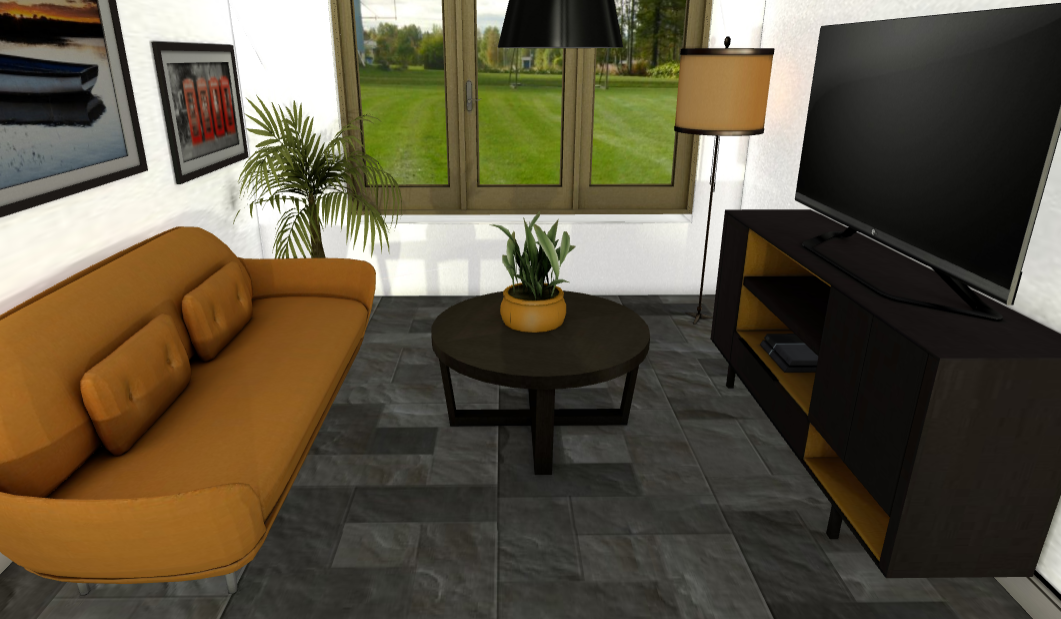
\includegraphics[width=1\linewidth]{images/chapter_baking_service/bake_no_luci.png}\hfill
 \caption[Scena processata dal servizio di bake ]{Scena processata dal servizio di bake in cui non sono presenti oggetti luce}
 \label{fig:baking_service_bake_no_luci}
\end{figure}
Le fonti luminose per questo motivo non vengono descritte all’interno del formato di scambio JSON4 in uscita da Blender  le luci, permettendo quindi di evitare il mapping delle luci inverso a quello effettuato durante l’importazione.
\\
La totale assenza delle luci rende inoltre superfluo mappare in modo accurato i materiali del Cycles render di Blender in quelli utilizzati da Three.js. 
Risulta infatti totalmente inutile calcolare il valore di reflectivity di un materiale se poi quest’ultimo non viene colpito da nessuna luce.
Per i motivi appena citati l’exporter io\_three è stato modificato affinchè non esportasse luci e non effettuasse il mapping dei materiali inverso a quello effettuato nell’importazione della scena.
\\
Il materiale di ogni oggetto che partecipa al bake viene infatti esportato come Phong a cui viene assegnato un valore fisso di reflectivity.
I materiali degli oggetti che non partecipano vengono invece esportati come \texttt{MeshBasic}.
Questi ultimi siccome non partecipano al bake non hanno assegnate le texture lightmap ma solamente la diffuse texture originali ottenute durante il caricamento della scena.
Prima di esaminare il motivo di questa esportazione è necessaria però una piccola precisazione. 
In Three.js quando un oggetto non viene colpito da una luce appare scuro in quanto non illuminato, esattamente come accade nella vita reale.
Questo però non accade per gli oggetti con associato un materiale \texttt{Phong} a cui vengono assegnate una lightmap e le corrispondenti normali.
\\
Questi appaiono visibili (illuminati) all’interno della scena anche se nessuna luce li colpisce.
\\
Questo comportamento è stato sfruttato in questo lavoro di tesi al fine di ottenere scene visivamente fotorealistiche in cui le luci sono assenti. L’assenza di queste comporta infatti un notevole incremento delle prestazioni generali del rendering Three.js.
È chiaro quindi come non fosse possibile assegnare agli oggetti che non partecipano al bake (senza lightmap) un materiale di tipo Phong, pena l’ottenimento di oggetti scuri.
L’unico modo per poter esportare corretamente gli oggetti con sole diffuse texture da Blender è assegnargli un materiale di tipo Mesh Basic. 
Il Mesh Basic Material risulta un tipo di materiale che non viene influenzato dalle luci, quindi gli oggetti a cui è associato risultano visibili anche se non colpiti da luci.
Questo ha permesso di rendere visibili all’interno della scena Three.js gli oggetti senza lightmap che non hanno subito il bake.
\\
\begin{figure}[htb]
 \centering
 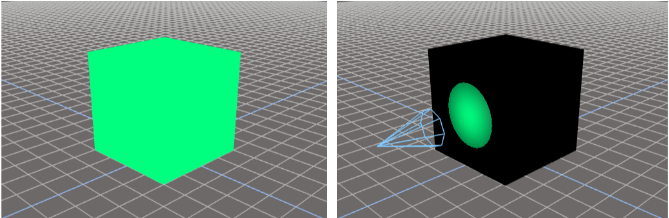
\includegraphics[width=1\linewidth]{images/chapter_baking_service/basic_phong.png}\hfill
 \caption[Differenza tra un materiale Basic ed uno Phong.]{A sinistra un materiale Basic non influenzato dalla luce, a destra uno Phong influenzato dalla luce.}
 \label{fig:baking_service_basic_phong}
\end{figure}

Nel presente lavoro di tesi agli oggetti che non devono subire il bake viene assegnato il parametro avoid\_bake e viene sfruttato soprattutto per le skybox, come spiegato nel paragrafo \ref{sec:chapter_baking_service_pipeline_baking_ciclo_bake}.
Nell’exporter in particolare per riconoscere se una texture è di tipo lightmap o di tipo diffuse sono state sfruttate le texture slot assegnate al materiale dell’oggetto. 
Viene ricordato come ad ogni texture slot viene assegnata una texture. In questo lavoro ogni materiale di un oggetto può avere due texture slot, uno per le diffuse ed uno per le lightmap.
Ad ogni texture slot è assegnato un parametro blend\_type con valore \texttt{ADD} nel caso in cui la texture associata sia una diffuse e \texttt{MULTIPLY} nel caso in cui sia una lightmap.
\\
Questi due texture slot sono stati sfruttati nell’exporter per identificare se ad un oggetto fossero o meno assegnate delle lightmap o diffuse texture.
Nel dettaglio quando viene esportato un oggetto con associata una lightmap, nel formato di scambio vengono trascritte le informazioni dell’immagine lightmap e vengono trascritte non solo le uv per la ligtmap ma anche le uv per la diffuse texture.
Questo di fatto permette a chi importa, nell’ambiente web, la scena con le lightmap di rimuovere le lightmap non desiderate per rimettere le vecchie diffuse texture.
\\ 
Le diffuse texture vengono inserite correttamente in quanto vengono sfruttate le uv per le diffuse texure inserite nel formato di scambio e poi associate all’oggetto Three.js.
Questo comportamento da parte dell’utilizzatore è molto raro che si verifichi, ma certo non impossibile, quindi è stata aggiunta questa possibilità in modo tale da rendere il tool più flessibile.
\\
Inoltre l’exporter originale causava problemi con l’esportazione del colore dei materiali provocando alle scene esportate uno smorzamento dei colori, come una patina grigia che le sovrastava.
\\
\begin{figure}[htb]
 \centering
 
\includegraphics[width=1\linewidth]{images/chapter_baking_service/grigio_chiaro.png}\hfill
 \caption[Miglioramenti nell'esportazione dei colori.]{A sinistra una scena con colori smorzati dall'exporter io\_three, a destra una scena esportata correttamente con l'exporter creato.}
 \label{fig:baking_service_grigio_chiaro}
\end{figure}
Questo errore era dovuto dal fatto che l’exporter, specifico per il Blender render, utilizzava dei parametri per prelevare il colore dai materiali differenti da quelli che in realtà vengono usati nel Cycles Render. Quindi nel nuovo exporter sono stati utilizzati i parametri corretti.
L’exporter infine non permetteva l’esportazione dell’ immagine applicata come texture. 
Il plug-in è stato quindi modificato affinchè lo permettesse.
\\
L’immagine assegnata all’oggetto, salvata in memoria principale di Blender, viene prelevata, convertita in base 64  e poi scritta all’interno del JSON 4 nel campo corrispondente.  
In Python la codifica può effettuata tramite l’utilizzo della funzione \texttt{b64encode(image\_file)} che accetta come parametro l’immagine da codificare. 
\\
Quelle appena presentate sono le principali modifiche effettuate nell’exporter, viene ora  mostrato come è stato utilizzato all’interno dello script creato in questo lavoro di tesi. 
\\
L’exporter può essere richiamato facilmente all’interno dello script creato per questo lavoro di tesi tramite l’utilizzo della funzione bpy.ops.export.three(filepath) che accetta come parametro il path locale di dove verrà salvato il JSON.
\\
Prima di richiamare questo plug-in sono necessari però un paio di accorgimenti.
Le normali originali dell’oggetto salvate in memoria durante la creazione della scena, mediante la struttura dati spiegata nel paragrafo \label{sec:chapter_baking_service_pipeline_baking_caricam_scena}, vengono sovrascritte a quelle ricalcolate da Blender. 
\\
Questo per permettere di osservare superfici smooth nella scena Three.js importata.
Inoltre viene effettuata una conversione di tutte le immagini in JPEG ed una successiva compressione di queste.
\\
Tutte le immagini .png vengono convertite in immagini .jpeg in quanto per definizione le lightmap non mappano trasparenze. Quindi esportare png sarebbe un inutile incremento di dimensione del JSON in quanto a differenza delle immagini jpeg occupano più spazio e la loro conversione comporta pochi benefici.
\\
La compressione in particolare  viene effettuata ad una qualità elevata, ma permette di diminuire enormemente la dimensione di immagini non compresse lasciando inalterata la qualità visiva.
Questo di fatto permette solitamente di ottenere scene nettamente inferiori di quelle arrivate come input al servizio, in alcuni casi si arriva addirittura ad un guadagno del 50\% di spazio. Quindi si ottengono scene molto più leggere e performanti da renderizzare.
\\
Dopo questi accorgimenti viene infine chiamato il plugin che effettua l’esportazione e la scena verrà scritta all’interno del JSON4 che verrà inviato tramite e-mail all’utente, come è stato spiegato nel capitolo \ref{cha:chapter_baking_service}.
\\
L’utilizzo del plugin io\_three come base ha quindi facilitato in questo lavoro di tesi la creazione dell’exporter da Blender Cycles render verso Three.js. 
Questo perchè molti degli adattamenti Blender Three.js classici, come la lettura dei vertici o delle facce del vecchio plugin (specifico per il Blender Render), erano anche validi per il Cycles render.